\documentclass[10pt]{beamer}
\usetheme{Boadilla}
\usepackage[T1]{fontenc}
\usepackage[latin1]{inputenc}
\usepackage{multimedia}
\usepackage{bbm}
\usepackage{array}
\usepackage{color}
\usepackage{graphicx}
\providecommand{\tabularnewline}{\\}

% Extension postscript
\usepackage{amsmath}
\usepackage{amsfonts}
\usepackage[english,french]{babel}
\usepackage[toc,page]{appendix} 
\usepackage{listings}
\usepackage{ifthen}
\usepackage{tabularx}
\usepackage{array}
\usepackage{subfigure}
\usepackage{rotating}

\newcommand\musec{\mu\text{s}}
\begin{document}
\title{IJK structured mesh implementation in Trio\_U}
\author{Benoit Mathieu}
\selectlanguage{english}
\begin{frame}
  \titlepage
\tableofcontents
\end{frame}
%===================================================================
\section{Data structures}
\begin{frame}[fragile]
\frametitle{Mesh geometry}
 The global mesh geometry is stored in the \verb|IJK_Grid_Geometry| class.
\begin{itemize}
\item Number of cells
\item Cells sizes (constant or not constant for each direction)
\item Periodicity flags
\end{itemize}
\only<1>{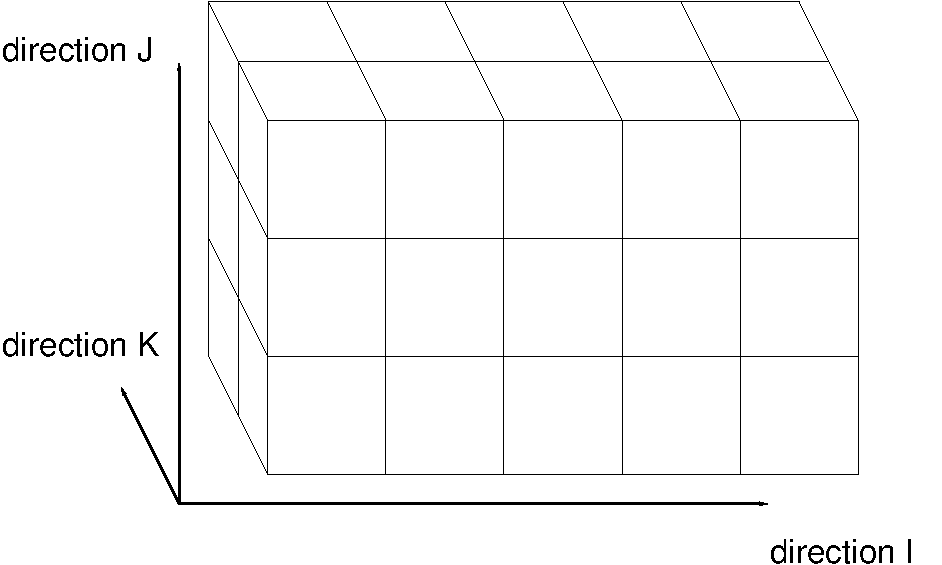
\includegraphics[width=10cm]{fig1}}
\only<2>{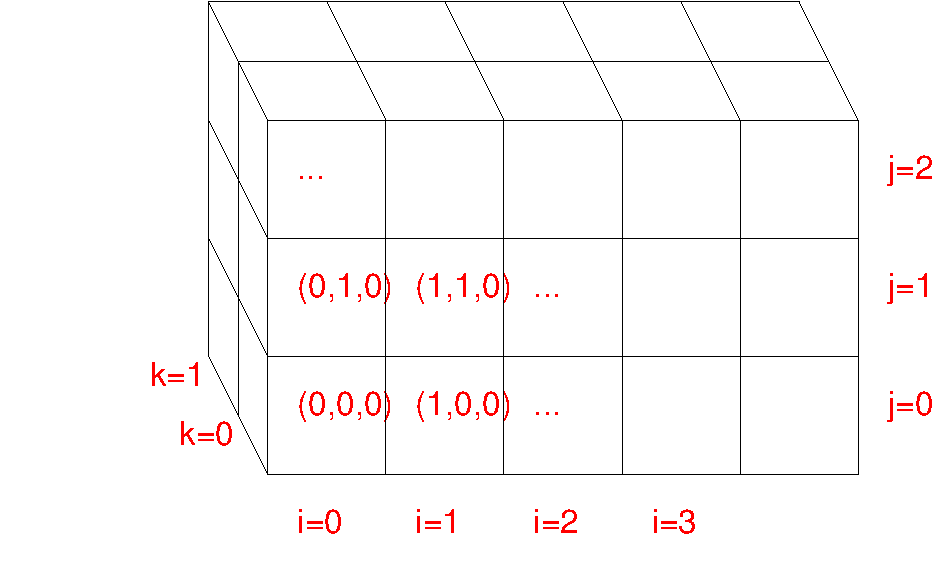
\includegraphics[width=10cm]{fig2}}

\end{frame}
%===================================================================
\begin{frame}[fragile]
\frametitle{Numbering of faces}
Face number (i,j,k) is at the ``left'' of element (i,j,k)

\only<1>{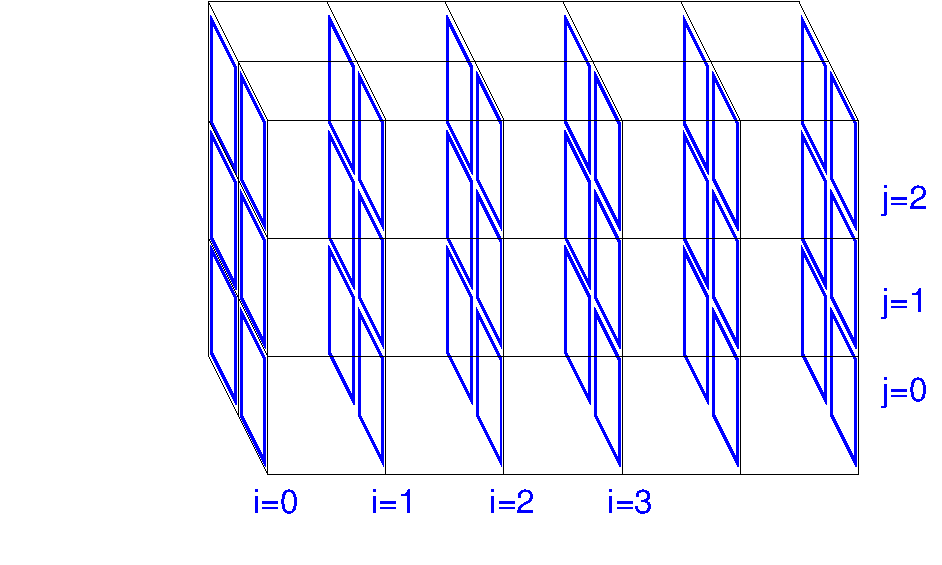
\includegraphics[width=10cm]{fig3}}
\only<2>{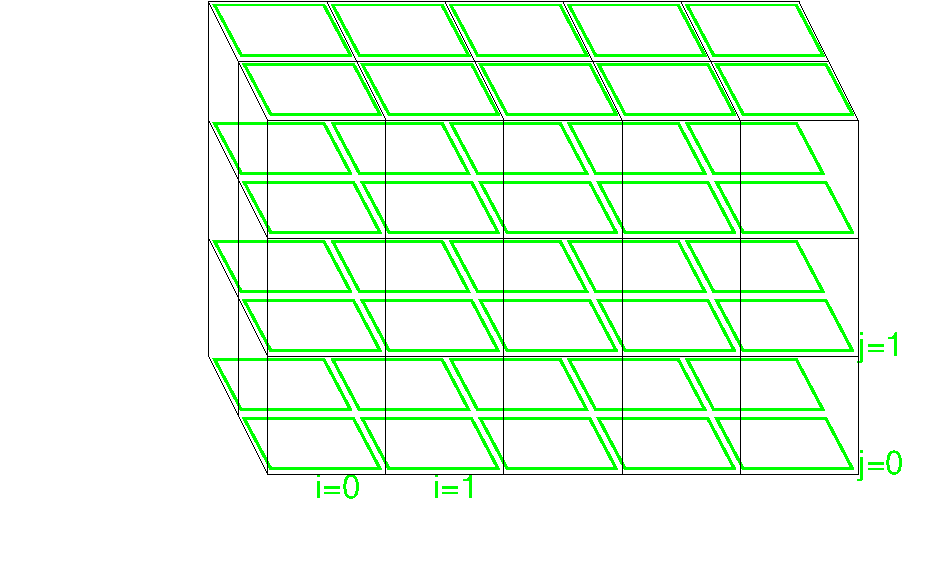
\includegraphics[width=10cm]{fig4}}
\only<3>{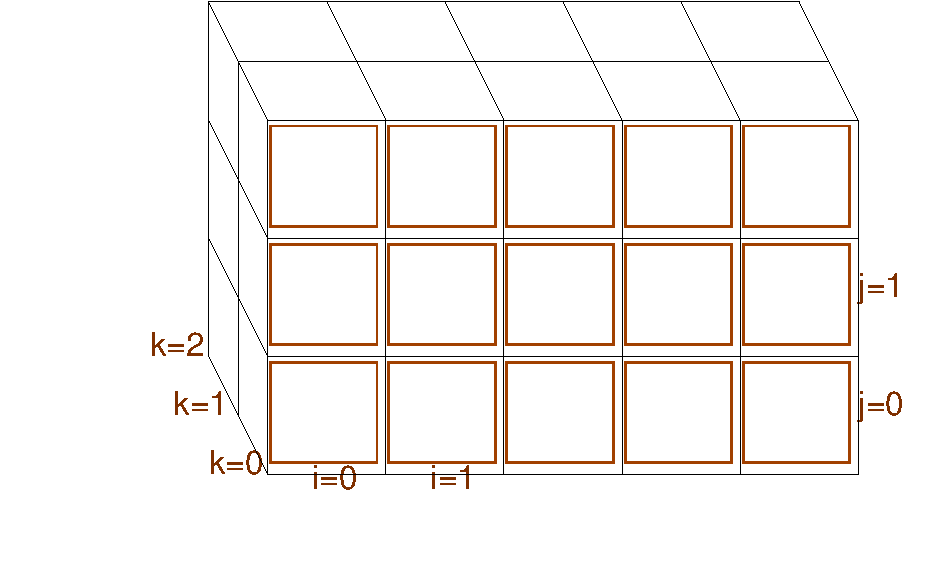
\includegraphics[width=10cm]{fig5}}
\end{frame}
%===================================================================
\begin{frame}[fragile]
\frametitle{Mesh splitting}
\begin{itemize}
  \item The partitionning of the mesh is provided by the \verb|IJK_Splitting| class.
  \item For the moment, only a ``structured'' splitting is supported (given number of
   slices in i, j, and k directions).
\end{itemize}
\only<1>{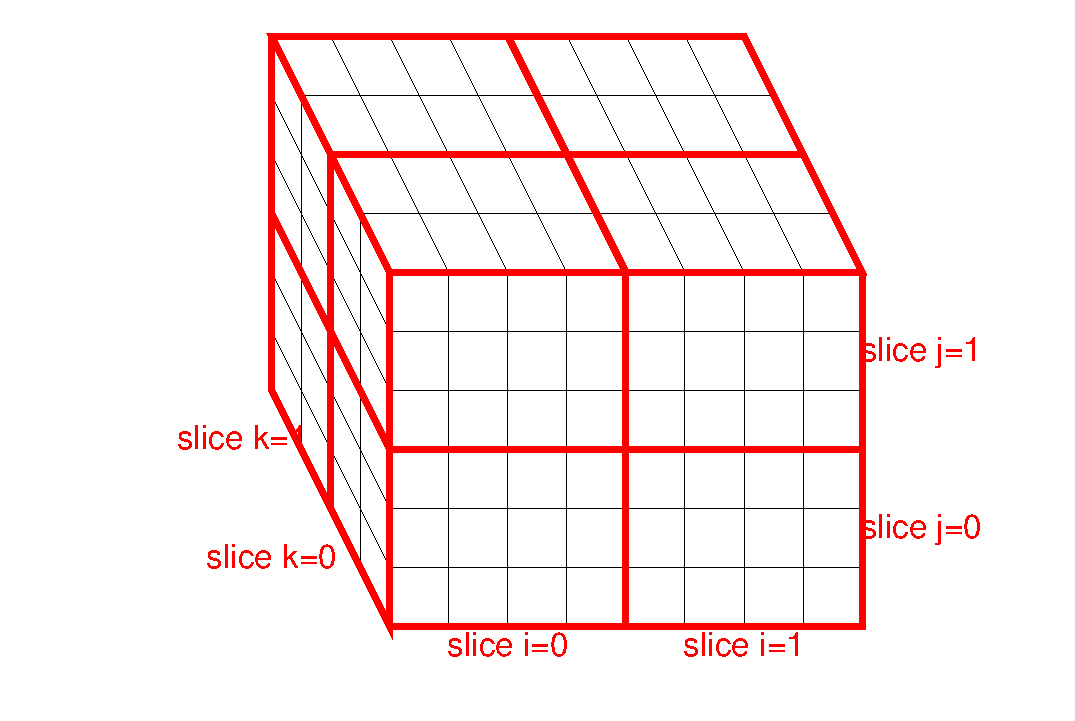
\includegraphics[width=8cm]{decoupage}}
\end{frame}
%===================================================================
\begin{frame}[fragile]
\frametitle{Splitting of elements}
\begin{itemize}
  \item Elements have local indices on each processor
  \item Global element/node/face index is obtained by addind the ``offset''
  \item Negative indices are ``ghost'' elements held by the neighbour processor
  \item Periodicity is handeled by ``ghost'' elements (even if there is only one slice)
\end{itemize}
\only<1>{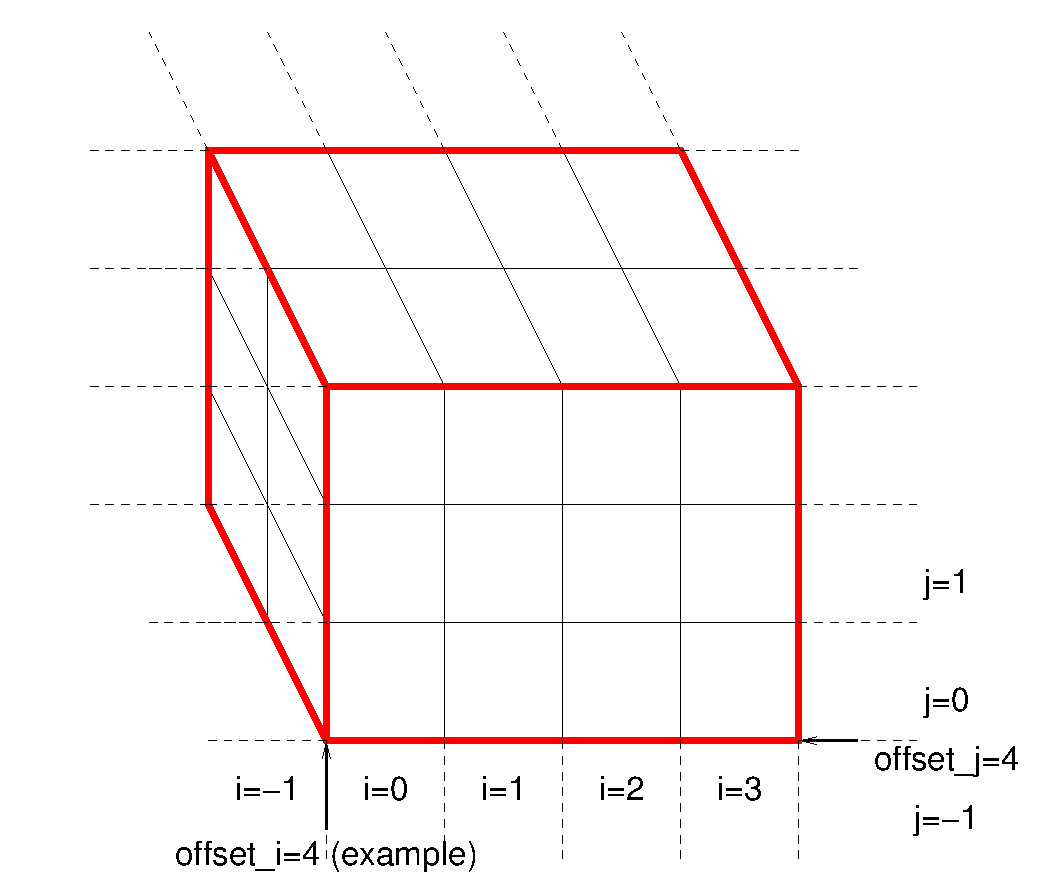
\includegraphics[width=7cm]{numero_local_elem}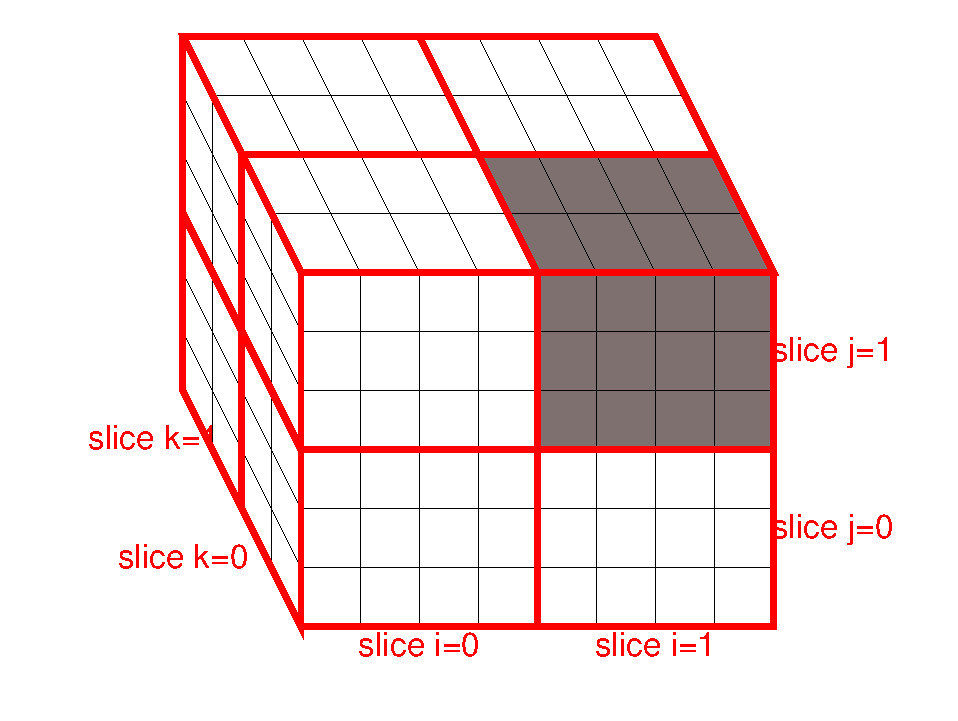
\includegraphics[width=5cm]{decoupage2}}
\end{frame}
%===================================================================
\begin{frame}[fragile]
\frametitle{Splitting of nodes and faces}
\begin{itemize}
  \item A node or a face belongs to one processor only
  \item The ``right'' face of the rightmost local element is a ``ghost'' face (except at
the boundary of the global domain if not periodic...)
  \item In the example, \verb|splitting.get_nb_faces_local(DIRECTION_I)| returns 4.
\end{itemize}
\only<1>{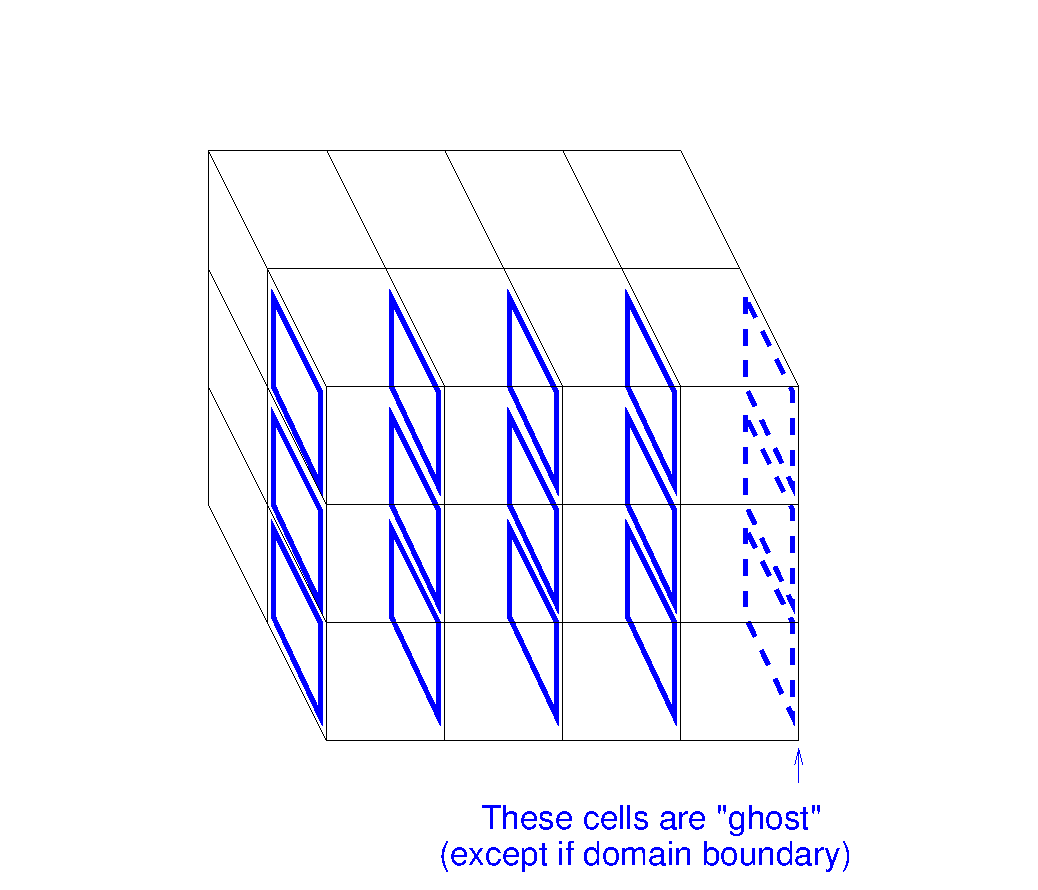
\includegraphics[width=7cm]{faces_locales}}
\end{frame}
%===================================================================
\begin{frame}[fragile]
\frametitle{Fields}
\begin{itemize}
  \item The \verb|IJK_Field_double| and \verb|IJK_Field_float| classes hold a field
    of scalar values localized on a split mesh.
  \item The following localizations are supported: ELEM, NODES, FACES\_I, FACES\_J, FACES\_K.
  \item On a processor, items are either ``real'' or ``ghost'' (but never ``common''):
    the node or face at the right of the last element on a processor is a ghost node or face;
    it is real on the processor that owns the next block of mesh cells.
\end{itemize}
\end{frame}


\end{document}